\documentclass{scrartcl}
\usepackage[utf8]{inputenc}
%\usepackage[T1]{fontenc}
\usepackage[a4paper, left=2.5cm, right=2.5cm, top=2.5cm, bottom=4cm]{geometry}
\usepackage[english]{babel}
\usepackage{amsmath, amsthm, amssymb, amstext}
\usepackage{listings}
\usepackage{color}
\usepackage{graphicx}
\usepackage{xparse}
\usepackage{fancyhdr}
\usepackage{algorithmicx}
\usepackage{algpseudocode}
\usepackage{algorithm}
\usepackage{parskip}
\usepackage[table]{xcolor}
\usepackage{tabularx}
\usepackage{enumerate}
\usepackage{enumitem}
%\usepackage{minted}
\usepackage {tikz}
\usetikzlibrary{positioning}

\pagestyle{fancy}


\rhead{{\newcommand\and\\\getauthors}}
\author{Felix Bühler\\2973410 \and Clemens Lieb\\3130838 \and Steffen Wonner\\2862123 \and Fabian Bühler\\2953320}
\lhead{\textbf\gettitle}
\title{\gettitle}
\chead{\getsubtitle}
\subtitle{\getsubtitle}

\addtolength{\headheight}{2\baselineskip}
\renewcommand{\headrulewidth}{0pt}

\newcommand{\gettitle}{Distributed systems I\\Winter Term 2019/20}
\newcommand{\getsubtitle}{G2T1 – Assignment 3 (theoretical part)}
\newcommand{\getauthors}{Felix Bühler \and Clemens Lieb \and Steffen Wonner \and Fabian Bühler}
\setlength{\headheight}{53pt}

\begin{document}
\maketitle

\section*{1 - Physical Clocks}
\subsection*{a)}

\begin{figure}[ht!]
\begin{tikzpicture}[scale=0.2]
\foreach \x in {1,...,81} {
	\draw (\x,0) -- (\x, 2);
	\draw (\x, -5) -- (\x, -7);
};
\draw (0,0) -- (81,0);
\draw (0,-5) -- (81,-5);
\node at(0, -1) {\tiny Master};
\node at(0, -4) {\tiny Slave};
\foreach \x/\n in {3/7,8/8,13/9,18/10,23/11,28/12,33/13,38/14,43/15,48/16,53/17,58/18,63/19,68/20,73/21,78/22} {
	\draw node[rectangle, fill=black, text width=1mm, inner sep=0, minimum height=4mm] at(\x,1) (a\n) {}
		node[below=7mm, above of=a\n] {\tiny \n};
};
\foreach \x/\n in {3/3,8/4,13/5,18/6,23/7,28/8,31/9,34/10,37/11,40/12,43/13,46/14,49/15,52/16,55/17,58/18,63/19,68/20,73/21,78/22} {
	\draw node[rectangle, fill=black, text width=1mm, inner sep=0, minimum height=4mm] at(\x,-6) (b\n) {}
		node[above=7mm, below of=b\n] {\tiny \n};
};
\path[draw,->] 
	(b5.north) edge (a10.south)
	(a11.south) edge (b8.north);
\end{tikzpicture}
\caption{Solution for Figure 1}
\end{figure}
\begin{align*}
O = \frac12((t_2 - t_1) - (t_4 - t_3)) = \frac12((10 - 5) - (8 - 11)) = \frac12(5 + 3) = 4 &\\
d = 1 & \\
\Delta = 6, C_s(t_4 + \Delta) = 18 & \\
\frac{dC_S}{dt} = \frac{6 + 4}{6} = \frac{5}{3} &
\end{align*}

\begin{figure}[ht!]
	\begin{tikzpicture}[scale=0.2]
	\foreach \x in {1,...,81} {
		\draw (\x,0) -- (\x, 2);
		\draw (\x, -5) -- (\x, -7);
	};
	\draw (0,0) -- (81,0);
	\draw (0,-5) -- (81,-5);
	\node at(0, -1) {\tiny Master};
	\node at(0, -4) {\tiny Slave};
	\foreach \x/\n in {3/1,8/2,13/3,18/4,23/5,28/6,33/7,38/8,43/9,48/10,53/11,58/12,63/13,68/14,73/15,78/16} {
		\draw node[rectangle, fill=black, text width=1mm, inner sep=0, minimum height=4mm] at(\x,1) (a\n) {}
			node[below=7mm, above of=a\n] {\tiny \n};
	};
	\foreach \x/\n in {3/6,8/7,13/8,18/9,23/10,28/11,41/12,55/13,68/14,73/15,78/16} {
		\draw node[rectangle, fill=black, text width=1mm, inner sep=0, minimum height=4mm] at(\x,-6) (b\n) {}
			node[above=7mm, below of=b\n] {\tiny \n};
	};
	\path[draw,->]
		(b8.north) edge (a4.south)
		(a5.south) edge (b11.north);
\end{tikzpicture}
\caption{Solution for Figure 2}
\end{figure}
\begin{align*}
O = \frac12((t_2 - t_1) - (t_4 - t_3)) = \frac12((4 - 8) - (11 - 5)) = \frac12(-4 - 6) = -5  &\\
d = 1 & \\
\Delta = 8, C_s(t_4 + \Delta) = 14 & \\
\frac{dC_S}{dt} = \frac{8 - 5}{8} = \frac{3}{8} &
\end{align*}

\subsection*{b)}
\begin{enumerate}[label=(\roman*)]

	\item We can use the difference in offsets to determine the clockrate of the master node in relation to the subservient node.
	For that purpose we calculate \(O_1 = \frac12((t_6 - t_5) - (t_8 - t_7))\) and \(O_0 = \frac12((t_2 - t_1) - (t_4 - t_3))\).
	
	It's clear that \(\frac{O_1 - O_0}{t_6 - t_2}\) is the rate at which the clocks are desynchronizing in reference to the master clock.
	If \(O_1 - O_0\) is negative, the subservient clock is faster than the master, and vice versa.
	This means that for negative \(O_1 - O_0\), the frequency ratio is \(f = \frac{t_6 - t_2}{O_0 - O_1}\).
	For a faster master clock the frequency ratio is the desynchronization rate from before.

	\item It makes no sense to synchronize the clock rates before the clock values, because to enable a ''stable'' value synchronization  -- i.e. monotonically increasing without large gaps in tick-time or clockvalues -- the clock frequency needs to be adjusted again.
	As such, the synchronized clock frequency would need to be changed again to synchronize clock values, making it an unnecessary step.

	\item Synchronization of the depicted clocks.
	\begin{align*}
		O_0 = \frac12((5-6)-(9-6)) = 1 & \\
		O_1 = \frac12((8-11) - (14-9)) = -4 & \\
		d = \frac12((8-11) + (14-9)) = 1 & \\
		f = \frac{(8 - 5)}{1 - (-4)} = \frac35 &
	\end{align*}

	We choose \(\Delta = 8, C_s(t_8 + \Delta) = 18\) modifying the clock frequency of \(C_s\) to \(f * \frac{\Delta + O_1}{\Delta}\) of the original frequency.
	When \(t_8 + \Delta\), we again modify the frequency by \(\frac{\Delta}{\Delta - O_1}\) to return to the synchronized clock freqency.
	
	This means \(\frac{dC_s}{dt} = f * \frac{8 - 4}{8} = f * \frac12 = \frac{3}{10}\)

	\item Completing the figure.
	\begin{figure}[ht!]
		\begin{tikzpicture}[scale=0.2]
		\foreach \x in {1,...,81} {
			\draw (\x,0) -- (\x, 2);
			\draw (\x, -5) -- (\x, -7);
		};
		\draw (0,0) -- (81,0);
		\draw (0,-5) -- (81,-5);
		\node at(0, -1) {\tiny Master};
		\node at(0, -4) {\tiny Slave};
		\foreach \x/\n in {3/4,8/5,13/6,18/7,23/8,28/9,33/10,38/11,43/12,48/13,53/14,58/15,63/16,68/17,73/18,78/19} {
			\draw node[rectangle, fill=black, text width=1mm, inner sep=0, minimum height=4mm] at(\x,1) (a\n) {}
				node[below=7mm, above of=a\n] {\tiny \n};
		};
		\foreach \x/\n in {3/5,6/6,9/7,12/8,15/9,18/10,21/11,24/12,27/13,30/14,40/15,50/16,60/17,70/18,75/19,80/20} {
			\draw node[rectangle, fill=black, text width=1mm, inner sep=0, minimum height=4mm] at(\x,-6) (b\n) {}
				node[above=7mm, below of=b\n] {\tiny \n};
		};
		\path[draw,->]
			(b6.north) edge (a5.south)
			(a6.south) edge (b9.north)
			(b11.north) edge (a8.south)
			(a9.south) edge (b14.north);
	\end{tikzpicture}
	\caption{Solution 1b)(iv)}
	\end{figure}

	Note that the delay is not used in the timing schema proposed in (i).
	It has been included in the calculations for (iii) for completeness' sake.
\end{enumerate}

\section*{2 - Logical Clocks}
\subsection*{a)}
\begin{enumerate}[label=(\roman*)]
	\item 
	C(e$^1_1$) = 2\\
	C(e$^2_1$) = 3\\
	C(e$^3_1$) = 4\\
	C(e$^4_1$) = 5\\

	C(e$^1_2$) = 5\\
	C(e$^2_2$) = 6\\
	C(e$^3_2$) = 7\\
	C(e$^4_2$) = 8\\

	C(e$^1_3$) = 1\\
	C(e$^2_3$) = 2\\
	C(e$^3_3$) = 3\\
	C(e$^4_3$) = 9\\
	\item 
	VC(e$^1_1$) = \texttt{[1 0 1]}\\
	VC(e$^2_1$) = \texttt{[2 0 1]}\\
	VC(e$^3_1$) = \texttt{[3 0 1]}\\
	VC(e$^4_1$) = \texttt{[4 0 1]}\\

	VC(e$^1_2$) = \texttt{[3 1 1]}\\
	VC(e$^2_2$) = \texttt{[3 2 2]}\\
	VC(e$^3_2$) = \texttt{[3 3 2]}\\
	VC(e$^4_2$) = \texttt{[3 4 2]}\\

	VC(e$^1_3$) = \texttt{[0 0 1]}\\
	VC(e$^2_3$) = \texttt{[0 0 2]}\\
	VC(e$^3_3$) = \texttt{[0 0 3]}\\
	VC(e$^4_3$) = \texttt{[3 4 4]}\\
	\item
	P$_1$: e$^1_1$ e$^2_1$ e$^3_1$\\
	P$_2$: e$^1_2$ e$^2_2$\\
	P$_3$: e$^1_3$ e$^2_3$\\
	The vector event time of those events is smaller than the vector event time of e$^3_2$. A smaller vector time means events are causally related.
\end{enumerate}
\subsection*{b)}
\begin{enumerate}[label=(\roman*)]
	\item 
	P$_1$: e$_6$ e$_5$ e$_9$ e$_4$ e$_8$ e$_{10}$\\
	P$_2$: e$_{12}$ e$_3$ e$_{13}$\\
	P$_3$: e$_{11}$ e$_7$ e$_1$ e$_2$\\
	\item 
	Local event: e$_5$ e$_9$ e$_3$ e$_1$ e$_{11}$\\
	Send event: e$_6$ e$_4$ e$_{10}$ e$_{12}$\\
	Recieve event:  e$_8$ e$_{13}$ e$_7$ e$_2$\\
\end{enumerate}

\section*{3 - Global State}
\subsection*{a)}
$ \{(e^{1}_{1}, e^{1}_{2}), (e^{2}_{1}, e^{2}_{2}), (e^{2}_{2}, e^{3}_{1}), (e^{4}_{1}, e^{3}_{2}), (e^{4}_{1}, e^{4}_{2}), (e^{5}_{1}, e^{5}_{2}), (e^{1}_{1}, e^{2}_{2}), (e^{2}_{2}, e^{4}_{1}), (e^{4}_{1}, e^{5}_{2})\} $

\subsection*{b)}
\begin{enumerate}
	\item yes, as it is a valid linearization.
	\item no, because $ e_{2}^{3} $ can not happen before $ e_{1}^{3} $
\end{enumerate}

\subsection*{c)}
\begin{figure}[!ht]
	\centering
	\begin{tikzpicture}[auto,node distance=1.5cm]
		\node[draw] (s00) {$ S_{00} $};
		\node[draw] (s10) [below left = of s00] {$ S_{10} $};
		\node[draw] (s01) [below right = of s00] {$ S_{01} $};
		\node[draw] (s11) [below right = of s10] {$ S_{11} $};
		\node[draw] (s02) [below right = of s01] {$ S_{02} $};
		
		\node[draw] (s21) [below left = of s11] {$ S_{21} $};
		\node[draw] (s12) [below left = of s02] {$ S_{12} $};
		
		\node[draw] (s31) [below left = of s21] {$ S_{31} $};
		\node[draw] (s22) [below left = of s12] {$ S_{22} $};
		
		\node[draw] (s41) [below left = of s31] {$ S_{41} $};
		\node[draw] (s32) [below left = of s22] {$ S_{32} $};
		
		\node[draw] (s42) [below right = of s41] {$ S_{42} $};
		\node[draw] (s33) [below right = of s32] {$ S_{33} $};
		
		\node[draw] (s43) [below right = of s42] {$ S_{43} $};
		\node[draw] (s34) [below right = of s33] {$ S_{34} $};
		
		\node[draw] (s44) [below right = of s43] {$ S_{44} $};
		\node[draw] (s35) [below right = of s34] {$ S_{35} $};
		
		\node[draw] (s54) [below left = of s44] {$ S_{54} $};
		\node[draw] (s45) [below left = of s35] {$ S_{45} $};
		
		\node[draw] (s55) [below right = of s54] {$ S_{55} $};
		
		\path (s10) edge node {$ e^{1}_{1} $} (s00);
		\path (s11) edge node {$ e^{1}_{1} $} (s01);
		\path (s12) edge node {$ e^{1}_{1} $} (s02);
		
		\path (s00) edge node {$ e^{1}_{2} $} (s01);
		\path (s10) edge node {$ e^{1}_{2} $} (s11);
		
		\path (s21) edge node {$ e^{2}_{1} $} (s11);
		\path (s22) edge node {$ e^{2}_{1} $} (s12);
		
		\path (s41) edge node {$ e^{2}_{2} $} (s42);
		\path (s31) edge node {$ e^{2}_{2} $} (s32);
		\path (s21) edge node {$ e^{2}_{2} $} (s22);
		\path (s11) edge node {$ e^{2}_{2} $} (s12);
		\path (s01) edge node {$ e^{2}_{2} $} (s02);
		
		\path (s31) edge node {$ e^{3}_{1} $} (s21);
		\path (s32) edge node {$ e^{3}_{1} $} (s22);
		
		\path (s32) edge node {$ e^{3}_{2} $} (s33);
		\path (s42) edge node {$ e^{3}_{2} $} (s43);
		
		\path (s41) edge node {$ e^{4}_{1} $} (s31);
		\path (s42) edge node {$ e^{4}_{1} $} (s32);
		\path (s43) edge node {$ e^{4}_{1} $} (s33);
		\path (s44) edge node {$ e^{4}_{1} $} (s34);
		\path (s45) edge node {$ e^{4}_{1} $} (s35);
		
		\path (s33) edge node {$ e^{4}_{2} $} (s34);
		\path (s43) edge node {$ e^{4}_{2} $} (s44);
		
		\path (s34) edge node {$ e^{5}_{2} $} (s35);
		\path (s44) edge node {$ e^{5}_{2} $} (s45);
		\path (s54) edge node {$ e^{5}_{2} $} (s55);
		
		\path (s54) edge node {$ e^{5}_{1} $} (s44);
		\path (s55) edge node {$ e^{5}_{1} $} (s45);
	\end{tikzpicture}
	\caption{solution for 3.c)}
\end{figure}

\newpage
\section*{4 - Snapshot Algorithm}
\subsection*{a)}

See Figure \ref{fig:4a}

\begin{figure}[!ht]
    \centering
    \begin{tikzpicture}[auto,node distance=1.5cm,event/.style={fill=black,circle, inner sep=0pt, minimum size=5pt},state/.style={draw,rectangle, red, color=red, inner sep=0pt, minimum size=5pt, minimum width=10pt}, msg/.style={-latex,thick}, marker/.style={-latex,thick,red}]
        \node[] (p1s) {\(P_1\)};
        \node[] (p2s) [below = of p1s] {\(P_2\)};
        \node[] (p3s) [below = of p2s] {\(P_3\)};
        
        \node[] (p1e) [right = 13cm of p1s] {};
        \node[] (p2e) [right = 13cm of p2s] {};
        \node[] (p3e) [right = 13cm of p3s] {};
        
        \path (p1s.east) edge (p1e);
        \path (p2s.east) edge (p2e);
        \path (p3s.east) edge (p3e);
        
        \node[event,label={\(e_1^1\)}] (e11) [right = 1.3cm of p1s] {};
        \node[event,label={\(e_2^1\)}] (e21) [right = 1cm of p2s] {};
        \node[event,label={\(e_3^1\)}] (e31) [right = 2cm of p3s] {};
        
        
        \node[event,label={\(e_1^2\)}] (e12) [right = 4.2cm of p1s] {};
        \node[event,label={\(e_2^2\)}] (e22) [right = 2.1cm of p2s] {};
        \node[event,label={\(e_3^2\)}] (e32) [right = 4cm of p3s] {};
        
        
        \node[event,label={\(e_1^3\)}] (e13) [right = 6cm of p1s] {};
        \node[event,label={\(e_2^3\)}] (e23) [right = 4.5cm of p2s] {};
        \node[event,label={\(e_3^3\)}] (e33) [right = 10cm of p3s] {};
        
        
        \node[event,label={\(e_1^4\)}] (e14) [right = 7cm of p1s] {};
        \node[event,label=below:{\(e_2^4\)}] (e24) [right = 8.5cm of p2s] {};
        
        
        \node[event,label={\(e_1^5\)}] (e15) [right = 10.5cm of p1s] {};
        \node[event,label={\(e_2^5\)}] (e25) [right = 9cm of p2s] {};
        
        \node[event,label={\(e_2^6\)}] (e26) [right = 12.5cm of p2s] {};
        
        \path (e21) edge[msg] node {\(m_1\)} (e31);
        \path (e11) edge[msg] node[left] {\(m_2\)} (e23);
        \path (e22) edge[msg] node[right] {\(m_3\)} (e12);
        \path (e32) edge[msg] node[below right] {\(m_4\)} (e14);
        \path (e13) edge[msg] node[right] {\(m_5\)} (e25);
        \path (e15) edge[msg] node {\(m_6\)} (e26);
        \path (e24) edge[msg] node {\(m_7\)} (e33);
        
        \node[state,label={[red]:{\(s_3\)}}] (s3) [right = 3cm of p3s] {};
        \node[state,label={[red]:{\(s_1,c_4\)}}] (s1) [right = 5cm of p1s] {};
        \node[state,label={[red]below:{\(s_2,c_1\)}}] (s2) [right = 6.5cm of p2s] {};
        
        \node[state,label={[red]:{\(c_2\)}}] (c2) [right = 8cm of p1s] {};
        \node[state,label={[red]:{\(c_3\)}}] (c3) [right = 8.5cm of p3s] {};
        
        \path (s3.north east) edge[marker] node[below] {\(M\)} (s1.south west);
        \path (s1.south east) edge[marker] node[left] {\(M'\)} (s2.north west);
        \path (s2.north east) edge[marker] node[below left] {\(M''\)} (c2.south west);
        \path (s2.south east) edge[marker] node[] {\(M''\)} (c3.north west);
    \end{tikzpicture}
    
    The red boxes represent where a process saves some state. A process state save is denoted by \(s_i\) and a channel state save by \(c_j\) where \(i\) is the process number and \(j\) is the channel number.
	\caption{solution for 4.a)}
	\label{fig:4a}
\end{figure}

\subsection*{b)}

No channel received a message between the process starting recording and the first/second marker arriving. All channel states are empty sets.

\begin{align*}
    c_1 &= \{\}\\
    c_2 &= \{\}\\
    c_3 &= \{\}\\
    c_4 &= \{\}\\
\end{align*}

\end{document}
